% ============================================================
%  YZV416E Computer Vision — Final Project Report
%  Topic E: Flow Estimation Robustness – RAFT vs GMFlow
%  Team: LetItFlow  |  Istanbul Technical University
% ============================================================
\documentclass[11pt,a4paper]{article}

\usepackage[a4paper, top=2.2cm, bottom=2.2cm, left=2.5cm, right=2.5cm]{geometry}
\usepackage{times}
\usepackage{amsmath,amssymb}
\usepackage{graphicx}
\usepackage{booktabs}
\usepackage{multirow}
\usepackage{caption}
\usepackage{subcaption}
\usepackage{hyperref}
\usepackage{xcolor}
\usepackage{enumitem}
\usepackage{microtype}
\usepackage{parskip}
\usepackage{placeins}  % provides \FloatBarrier

% Keep floats within their section
\makeatletter
\AtBeginDocument{%
  \let\origsection\section
  \renewcommand{\section}{\FloatBarrier\origsection}
}
\makeatother

\hypersetup{colorlinks=true, linkcolor=blue!70!black, citecolor=blue!70!black, urlcolor=blue!70!black}

\setlength{\parskip}{4pt}
\setlength{\parindent}{0pt}

% ---- helpers ----
\newcommand{\raft}{RAFT-32}
\newcommand{\basic}{GMFlow-basic}
\newcommand{\refine}{GMFlow-refine}
\newcommand{\epe}{\text{EPE}}

% ============================================================
\begin{document}
% ============================================================

% ---- Title block ----
\begin{center}
  {\Large\bfseries YZV416E Computer Vision}\\[4pt]
  {\large Istanbul Technical University}\\[2pt]
  {\normalsize Department of AI and Data Engineering /
  Faculty of Computer and Informatics Engineering}\\[4pt]
  {\large\bfseries Final Project Report Submission --- Spring 2026 Term}
\end{center}

\vspace{6pt}
\noindent\rule{\linewidth}{0.6pt}
\vspace{4pt}

\noindent
\begin{tabular}{@{}ll}
\textbf{Selected Topic:} & E --- Flow Estimation Robustness: RAFT vs GMFlow \\[3pt]
\textbf{Instructor:}     & Prof.~Dr.~G\"{o}zde \"{U}nal \\[3pt]
\textbf{Team Name:}      & LetItFlow \\[3pt]
\textbf{Team Members:}   &
  \begin{tabular}[t]{@{}l@{\quad}l@{\quad}l@{\quad}l}
    Emin Acar            & AI \& Data Eng. & Model pipeline, data curation   & \\ 150220316 & acarme22@itu.edu.tr \\
    Batuhan Berk Balc\i  & AI \& Data Eng. & Model pipeline, evaluation      & \\ 150230330 & balcib23@itu.edu.tr \\
    Hasan Y.\ Ar{\i}kano\u{g}lu & AI \& Data Eng. & Model pipeline, report writing & \\ 150220341 & arikanoglu22@itu.edu.tr \\
  \end{tabular} \\[3pt]
\textbf{Model Used:}     & RAFT , GMFlow-basic, GMFlow-refine \\
\end{tabular}

\vspace{4pt}
\noindent\rule{\linewidth}{0.6pt}
\vspace{6pt}

% ============================================================
\section{Project Overview}
% ============================================================

We tackle \textbf{dense optical flow estimation}: predicting a per-pixel
2-D motion field $(u,v)$ that maps every pixel in frame $t$ to its location
in frame $t{+}1$.  Our study follows \textbf{Topic E — Flow Estimation
Robustness}: we take two published, frozen networks — RAFT
\cite{teed2020raft} and GMFlow \cite{xu2022gmflow} — and evaluate them
in a \emph{zero-shot} setting (Things-trained checkpoints, no Sintel or
Middlebury fine-tuning) on MPI-Sintel \cite{butler2012sintel} and the
Middlebury benchmark \cite{baker2011}.

\textbf{Why this is challenging:}
Optical flow is classically ill-posed (the aperture problem~\cite{horn1981}), and deep
models resolve it via fundamentally different mechanisms. RAFT builds
a 4-D all-pairs correlation volume and refines iteratively via ConvGRU.
GMFlow reformulates flow around Transformer-based feature enhancement,
global correlation/softmax matching, propagation, and optional refinement.
These architectures make opposite engineering bets — iterative local
refinement vs.\ global matching with propagation — which makes them the
natural pair to compare across
failure regimes: motion discontinuities, large displacements,
occlusions, textureless regions, and photometric degradations (the
Sintel Final pass adds motion blur, defocus, and atmospheric effects).

\textbf{Datasets:}
MPI-Sintel (training split) provides 1\,041 frame pairs per pass across
23 sequences at $1024{\times}436$ px, with ground-truth flow,
occlusion, and invalidity masks.  We evaluate on both Clean and Final
passes.  Middlebury provides 8 real-world sequence pairs with GT for
cross-dataset generalization.

\textbf{Main objectives:}
\begin{enumerate}[leftmargin=1.4em,topsep=2pt,itemsep=1pt]
  \item Evaluate zero-shot performance across 11 per-region masks
        (speed buckets, occlusion, motion boundaries, textureless,
        blur).
  \item Characterize where each architecture succeeds and fails via
        10 testable hypotheses with bootstrap confidence intervals.
  \item Quantify the accuracy-vs-latency trade-off via an RAFT
        iteration sweep and a three-way ablation with GMFlow's
        with-refinement variant.
\end{enumerate}

% ============================================================
\section{Model Architecture and System Overview}
% ============================================================

\subsection{RAFT}
RAFT \cite{teed2020raft} extracts features with a shared encoder, builds
a 4-D all-pairs correlation volume at multiple scales, and runs a
recurrent ConvGRU that iteratively looks up the volume and updates a
flow field.  Sub-pixel accuracy comes from the many refinement passes;
sharp boundaries come from the local correlation structure.
Checkpoint: \texttt{raft-things.pth} (Things-trained).
Inference with $k$ iterations: we sweep $k\in\{4,8,12,32\}$ with 32 as
the headline.

\subsection{GMFlow}
GMFlow \cite{xu2022gmflow} replaces iterative local refinement with a
global matching pipeline: Transformer-enhanced features are compared
through correlation and softmax matching, then refined through propagation.
A with-refinement variant adds a second-scale residual refinement stage.
Global matching helps with large displacement capture, while the attention
and correlation components increase memory and runtime pressure at higher
spatial resolutions.


\subsection{Pipeline and component table}
All inference uses the \texttt{cvflow} wrapper library
(\texttt{src/cvflow/}).  Inputs are padded to a multiple of the
model's required factor (RAFT: 8, GMFlow-basic: 16, GMFlow-refine: 32)
via replicate padding (\texttt{InputPadder}), and cropped back after
inference.  No fine-tuning; all backbone weights are frozen.

\begin{table}[htbp]
\centering
\caption{Pipeline component summary.}
\label{tab:components}
\setlength{\tabcolsep}{5pt}
\small
\begin{tabular}{llll}
\toprule
Module & Type & Status & Notes \\
\midrule
Image Encoder & Pretrained CNN & Frozen & Feature extraction \\
RAFT ConvGRU & Pretrained RNN & Frozen & Iterative refinement \\
GMFlow Transformer & Pretrained ViT & Frozen & Global matching \\
InputPadder & Custom & — & Resolution alignment \\
\midrule
All components & — & \textbf{Frozen} & Inference-only study \\
\bottomrule
\end{tabular}
\end{table}

% ============================================================
\section{Methodology and Experimental Setup}
% ============================================================

\subsection{Zero-shot framing and checkpoint selection}
We use Things-trained checkpoints exclusively (\texttt{raft-things} and
\texttt{gmflow\_things}).  Sintel-finetuned variants are available but
deliberately excluded: our hypothesis H10 tests cross-dataset
generalization from Sintel to Middlebury, which requires that neither
model has seen Sintel labels.  Using Sintel-finetuned weights would
contaminate this claim.

\subsection{Inference configuration}
\textbf{RAFT:} 32 iterations (headline), also swept at 4/8/12 for the
Pareto analysis.  \textbf{GMFlow-basic:} \texttt{attn\_splits=[2]},
\texttt{corr\_radius=[-1]}, \texttt{prop\_radius=[-1]},
\texttt{padding\_factor=16}.  \textbf{GMFlow-refine:} two-scale
attention, \texttt{padding\_factor=32}.  Hardware: NVIDIA RTX 3050 Ti
Laptop (4 GB), Python 3.11, PyTorch 2.6.0+cu124.

\subsection{Three-model ablation design}
The original RAFT-32 vs.\ GMFlow-basic comparison is
\emph{capacity-asymmetric}: GMFlow ships a with-refinement variant
(\refine) designed for parity with RAFT-32 in latency.  We therefore
run all analyses as a \textbf{three-way comparison} (RAFT-32,
GMFlow-basic, GMFlow-refine) so that any "RAFT wins vs.\ basic" result
can be checked against whether it holds vs.\ the capacity-matched
variant.

\subsection{Failure-region masks}
We derive five failure-region masks following Baker et al.\ \cite{baker2011}:
\begin{itemize}[leftmargin=1.4em,topsep=2pt,itemsep=1pt]
  \item \textbf{Disc} (motion boundaries): $\|\nabla u\|_1+\|\nabla v\|_1 > 1.0$ on GT flow, 9×9 dilation.
  \item \textbf{Untex} (textureless): $\|\nabla I\| < 5.0$, 3×3 dilation.
  \item \textbf{Blur}: windowed Laplacian variance $< 20$, 7×7 window.
  \item \textbf{Matched / Unmatched}: from Sintel occlusion masks.
  \item \textbf{Speed buckets}: $s_{0\text{-}10}$, $s_{10\text{-}40}$, $s_{40+}$, $s_{60+}$ (px/frame).
\end{itemize}

\subsection{Statistical testing}
Close EPE differences are tested with a paired sequence-level bootstrap
($n_\text{boot}=10{,}000$ resamples of the 23 Sintel sequences, 95\%
CIs).  Cells whose CI crosses zero are marked \textbf{NULL}; only
strongly significant cells ($|\Delta|/ \text{CI half-width} > 3$)
are relied on for hypothesis verdicts.  Because many mask/metric
comparisons are tested, bootstrap confidence intervals are interpreted
descriptively; no multiplicity correction is applied, so borderline effects
are not used as primary evidence.

% ============================================================
\section{Evaluation Metrics}
% ============================================================

\begin{table}[htbp]
\centering
\caption{Metrics used in this study.}
\label{tab:metrics}
\small
\setlength{\tabcolsep}{4pt}
\begin{tabular}{lp{6.5cm}}
\toprule
Metric & Description \\
\midrule
EPE & End-point error $\|\hat{f}-f^*\|_2$ (primary metric) \\
AE & Angular error; downweights large-motion errors \cite{baker2011} \\
Bad-$k$ & Fraction of pixels with EPE~$> k$~px ($k\in\{1,3,5,10\}$) \\
A50/A75/A95 & EPE percentile accuracies \\
nEPE & $\text{EPE}/|f^*|$ on pixels with $|f^*|>1$~px \\
Boundary F1 & F-score between pred.\ and GT flow edge maps, tol.\ 2~px \\
R0.5/R1.0/R2.0 & Middlebury robustness thresholds \\
Latency / VRAM & Median wall-clock (ms) and peak GPU memory (MB) \\
\bottomrule
\end{tabular}
\end{table}

EPE is the primary headline.  AE is reported for comparison with Baker
et al.\ \cite{baker2011} but treated as secondary because it
downweights large-motion failures.  Bad-1 px and A50 are the most
diagnostic distributional metrics.

% ============================================================
\section{Results and Analysis}
% ============================================================

\subsection{Sanity gate}
Before running the full evaluation we verified the pipeline against
published zero-shot Sintel numbers.  RAFT measured EPE
$1.4459$ (target $1.43$, $+1.1\%$) and $2.6779$ (target $2.71$,
$-1.2\%$); GMFlow measured $1.4839$ (target $1.495$, $-0.7\%$) and
$2.9420$ (target $2.955$, $-0.4\%$).  All within $\pm10\%$; pipeline
validated end-to-end.

\subsection{Sintel: main RAFT vs.\ GMFlow-basic table}

\begin{table}[htbp]
\centering
\caption{Sintel EPE on key masks.  \textbf{Bold}: lowest per column.
  \S: statistically NULL at 95\% bootstrap CI (ours vs.\ basic).
  Both shown checkpoints are Things-trained; no Sintel fine-tuning.}
\label{tab:sintel_main}
\small
\setlength{\tabcolsep}{4pt}
\begin{tabular}{lcccc}
\toprule
 & \multicolumn{2}{c}{\textbf{Clean}} & \multicolumn{2}{c}{\textbf{Final}} \\
\cmidrule(lr){2-3}\cmidrule(lr){4-5}
Mask & RAFT & GMFlow-b & RAFT & GMFlow-b \\
\midrule
All       & \textbf{1.446}\S & 1.484\S  & \textbf{2.678}\S & 2.942\S \\
Matched   & \textbf{0.646}   & 0.822    & \textbf{1.585}   & 1.902   \\
Unmatched & 11.69            & \textbf{9.95} & 16.67\S    & \textbf{16.25}\S \\
$s_{0\text{-}1}$  & \textbf{0.161} & 0.245 & \textbf{0.293} & 0.371 \\
$s_{40+}$ & 8.72\S & \textbf{8.19}\S & \textbf{17.41}\S & 17.63\S \\
$s_{60+}$ & 12.30\S & \textbf{11.21}\S & \textbf{23.61}\S & 23.84\S \\
Disc      & 3.58\S & \textbf{3.46}\S & \textbf{6.26}\S & 6.79\S \\
Untex     & 1.65\S & \textbf{1.55}\S & \textbf{3.11}\S & 3.46\S \\
Blur      & 2.18\S & \textbf{1.88}\S & \textbf{4.03}\S & 4.67\S \\
\midrule
Bad-1     & \textbf{0.098} & 0.160 & \textbf{0.147} & 0.209 \\
B-F1      & \textbf{0.727} & 0.697 & \textbf{0.698} & 0.672 \\
A50 (px)  & \textbf{0.067} & 0.411 & \textbf{0.068} & 0.409 \\
\bottomrule
\end{tabular}
\end{table}

\textbf{Key reads from Table~\ref{tab:sintel_main}.}
The headline ``RAFT EPE 1.446 vs.\ GMFlow-basic 1.484'' is
\emph{not significant} (95\% CI $[-0.19,+0.20]$, $p=0.64$).  RAFT's
clearest differences are on \emph{matched} pixels ($+0.177$, CI $[+0.058,+0.256]$)
and sub-pixel accuracy ($s_{0\text{-}1}$: $+0.084$, CI
$[+0.059,+0.131]$).  GMFlow-basic's clearest difference is on
\emph{unmatched}/occluded pixels ($-1.74$, CI $[-3.32,-0.12]$).
Nearly all large-motion and Disc/Untex comparisons are within
23-sequence noise.

The A50 column is particularly diagnostic: RAFT's median pixel error is
$0.067$~px; GMFlow-basic's is $0.411$~px — a $6\times$ gap.  This
traces to a coarse-grid ($k/8$) upsample residual in GMFlow's convex
upsampling: on \texttt{alley\_2}, 13\% of GMFlow-basic matched pixels
land within 0.02~px of the $2/8=0.25$ multiple (vs.\ $<1\%$ for RAFT).

\begin{figure}[!t]
  \centering
  \begin{subfigure}[t]{0.32\linewidth}
    \centering
    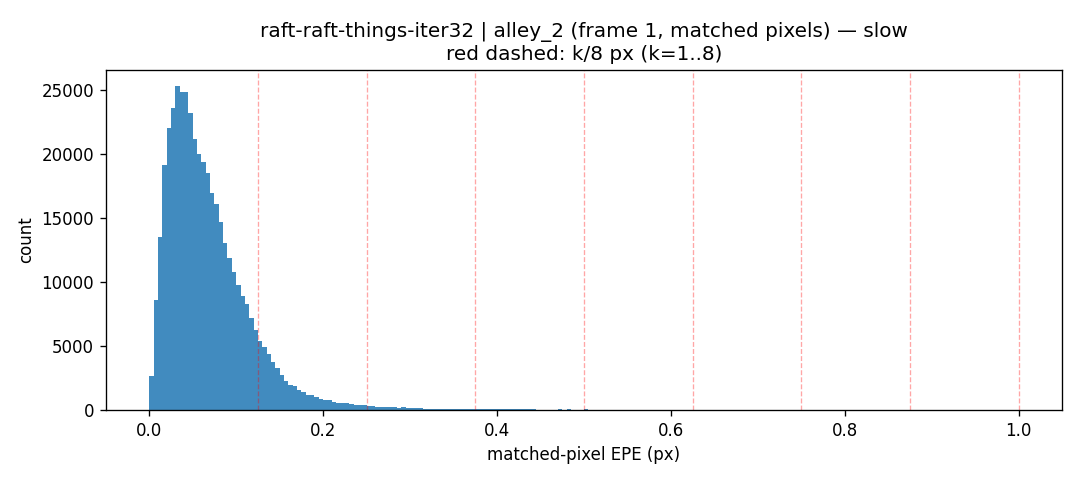
\includegraphics[width=\linewidth]{figures/quant_raft_alley2.png}
    \caption{RAFT-32}
  \end{subfigure}
  \hfill
  \begin{subfigure}[t]{0.32\linewidth}
    \centering
    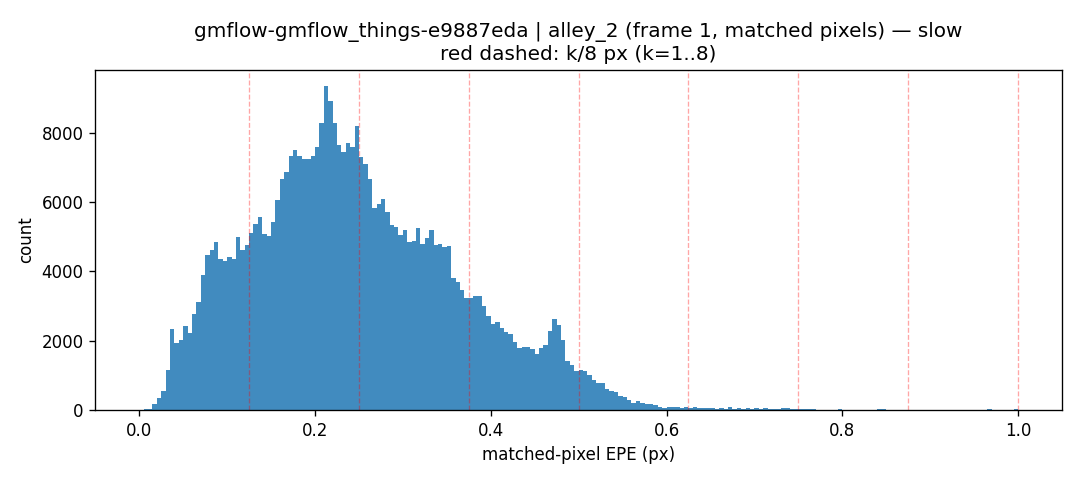
\includegraphics[width=\linewidth]{figures/quant_gmflow_basic_alley2.png}
    \caption{GMFlow-basic}
  \end{subfigure}
  \hfill
  \begin{subfigure}[t]{0.32\linewidth}
    \centering
    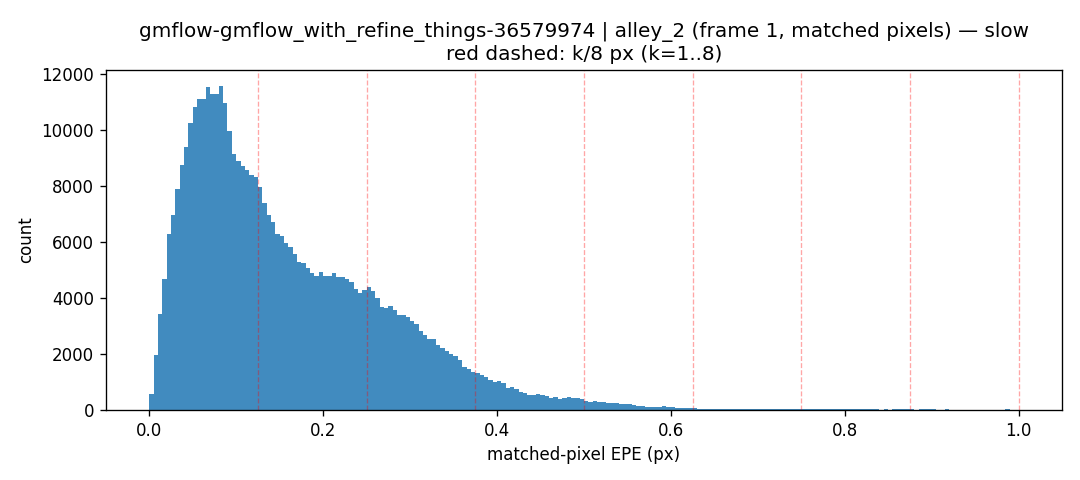
\includegraphics[width=\linewidth]{figures/quant_gmflow_refine_alley2.png}
    \caption{GMFlow-refine}
  \end{subfigure}
  \caption{Matched-pixel EPE histograms on a slow Sintel sequence
    (\texttt{alley\_2}).  Red dashed lines mark $k/8$-pixel residuals;
    GMFlow-basic has a visible concentration around the $2/8$ multiple,
    refine shifts the error mass lower, and RAFT is concentrated closest
    to zero.}
  \label{fig:quantization}
\end{figure}

\subsection{GMFlow-refine ablation}

Adding the with-refinement preset dramatically changes the picture
(Table~\ref{tab:refine}).  GMFlow-refine achieves EPE $1.073$ on
Sintel Clean — a 26\% improvement over RAFT-32 at only 10\% higher
latency.  On clean-pass EPE, the sequence bootstrap shows significant
refine wins on most masks, while $s_{0\text{-}1}$ and
$s_{0\text{-}10}$ are statistically tied (NULL).  Thus RAFT's sub-pixel
lead over GMFlow-basic largely disappears against the higher-capacity
GMFlow configuration.

\begin{table}[htbp]
\centering
\caption{Three-way EPE comparison, Sintel Clean.}
\label{tab:refine}
\small
\setlength{\tabcolsep}{5pt}
\begin{tabular}{lcccc}
\toprule
Mask & RAFT-32 & GMFlow-b & GMFlow-r & Winner \\
\midrule
All       & 1.446 & 1.484 & \textbf{1.073} & Refine \\
Matched   & 0.646 & 0.822 & \textbf{0.508} & Refine \\
Unmatched & 11.69 & 9.95  & \textbf{8.30}  & Refine \\
$s_{40+}$ & 8.72  & 8.19  & \textbf{6.19}  & Refine \\
Disc      & 3.58  & 3.46  & \textbf{2.54}  & Refine \\
B-F1      & 0.727 & 0.697 & \textbf{0.757} & Refine \\
A50 (px)  & \textbf{0.067} & 0.411 & 0.133 & RAFT \\
\bottomrule
\end{tabular}
\end{table}

The refine ablation suggests that several apparent RAFT advantages over
GMFlow-basic are better explained as capacity/configuration effects than
as purely architectural differences.  Only RAFT's A50 ($0.067$~px vs.\
$0.133$~px) persists — the coarse-grid upsample residual is reduced but
not eliminated by the refinement pass.

\subsection{Accuracy–latency trade-off}

\begin{figure}[!t]
  \centering
  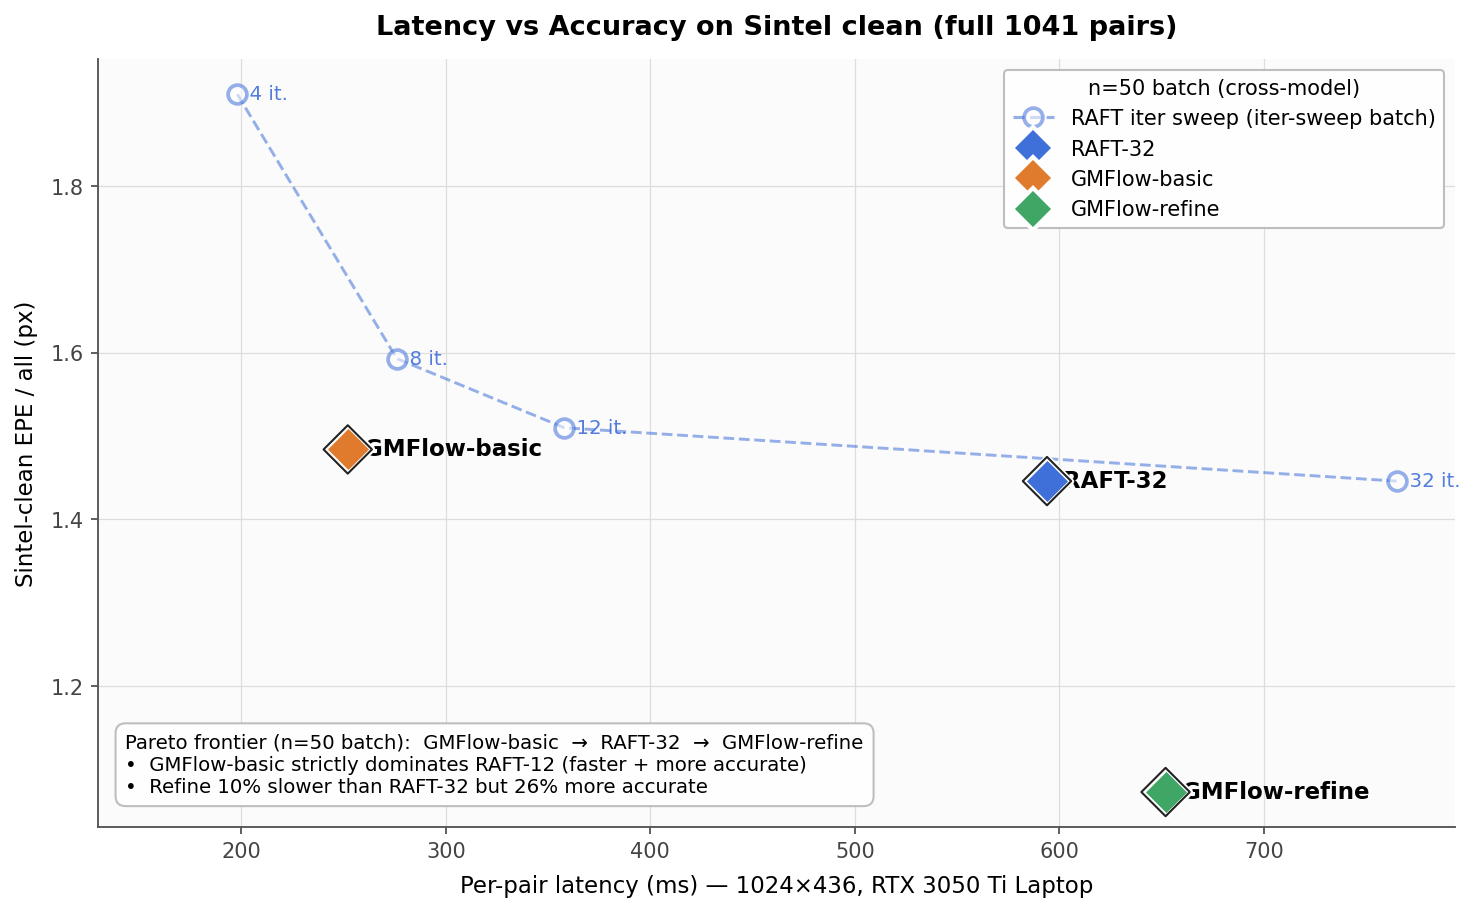
\includegraphics[width=0.80\linewidth]{figures/pareto.png}
  \caption{Pareto frontier: Sintel-Clean EPE vs.\ median latency (ms)
    at $1024{\times}436$.  Curve = RAFT iter sweep; markers = n=50
    cross-model batch.  GMFlow-basic appears to dominate RAFT-12; refine and
    RAFT-32 both sit on the frontier with refine at the accuracy corner.}
  \label{fig:pareto}
\end{figure}

The RAFT iteration sweep on all 23 sequences yields EPE
$1.910 / 1.593 / 1.510 / 1.446$ at $4/8/12/32$ iters with latencies
$198/276/358/765$~ms (iter-sweep batch).  Returns diminish sharply:
$4{\to}8$ iters saves 0.32 EPE for 78~ms; $12{\to}32$ saves only 0.06
EPE for 407~ms.

In the cross-model $n{=}50$ batch (same GPU thermal state for all
three): RAFT-32 = 594~ms / 529~MB VRAM;
GMFlow-basic = 252~ms / 470~MB;
GMFlow-refine = 652~ms / 1333~MB.
GMFlow-basic appears to dominate RAFT-12 (faster \emph{and} more
accurate, noting that the timing runs were separate).  Refine is 10\% slower
and 2.5$\times$ more VRAM-hungry than RAFT-32 while being 26\% more
accurate, so it is the better choice when accuracy is prioritized and
the memory budget is available.

\subsection{Per-region EPE and failure modes}

\begin{figure}[!t]
  \centering
  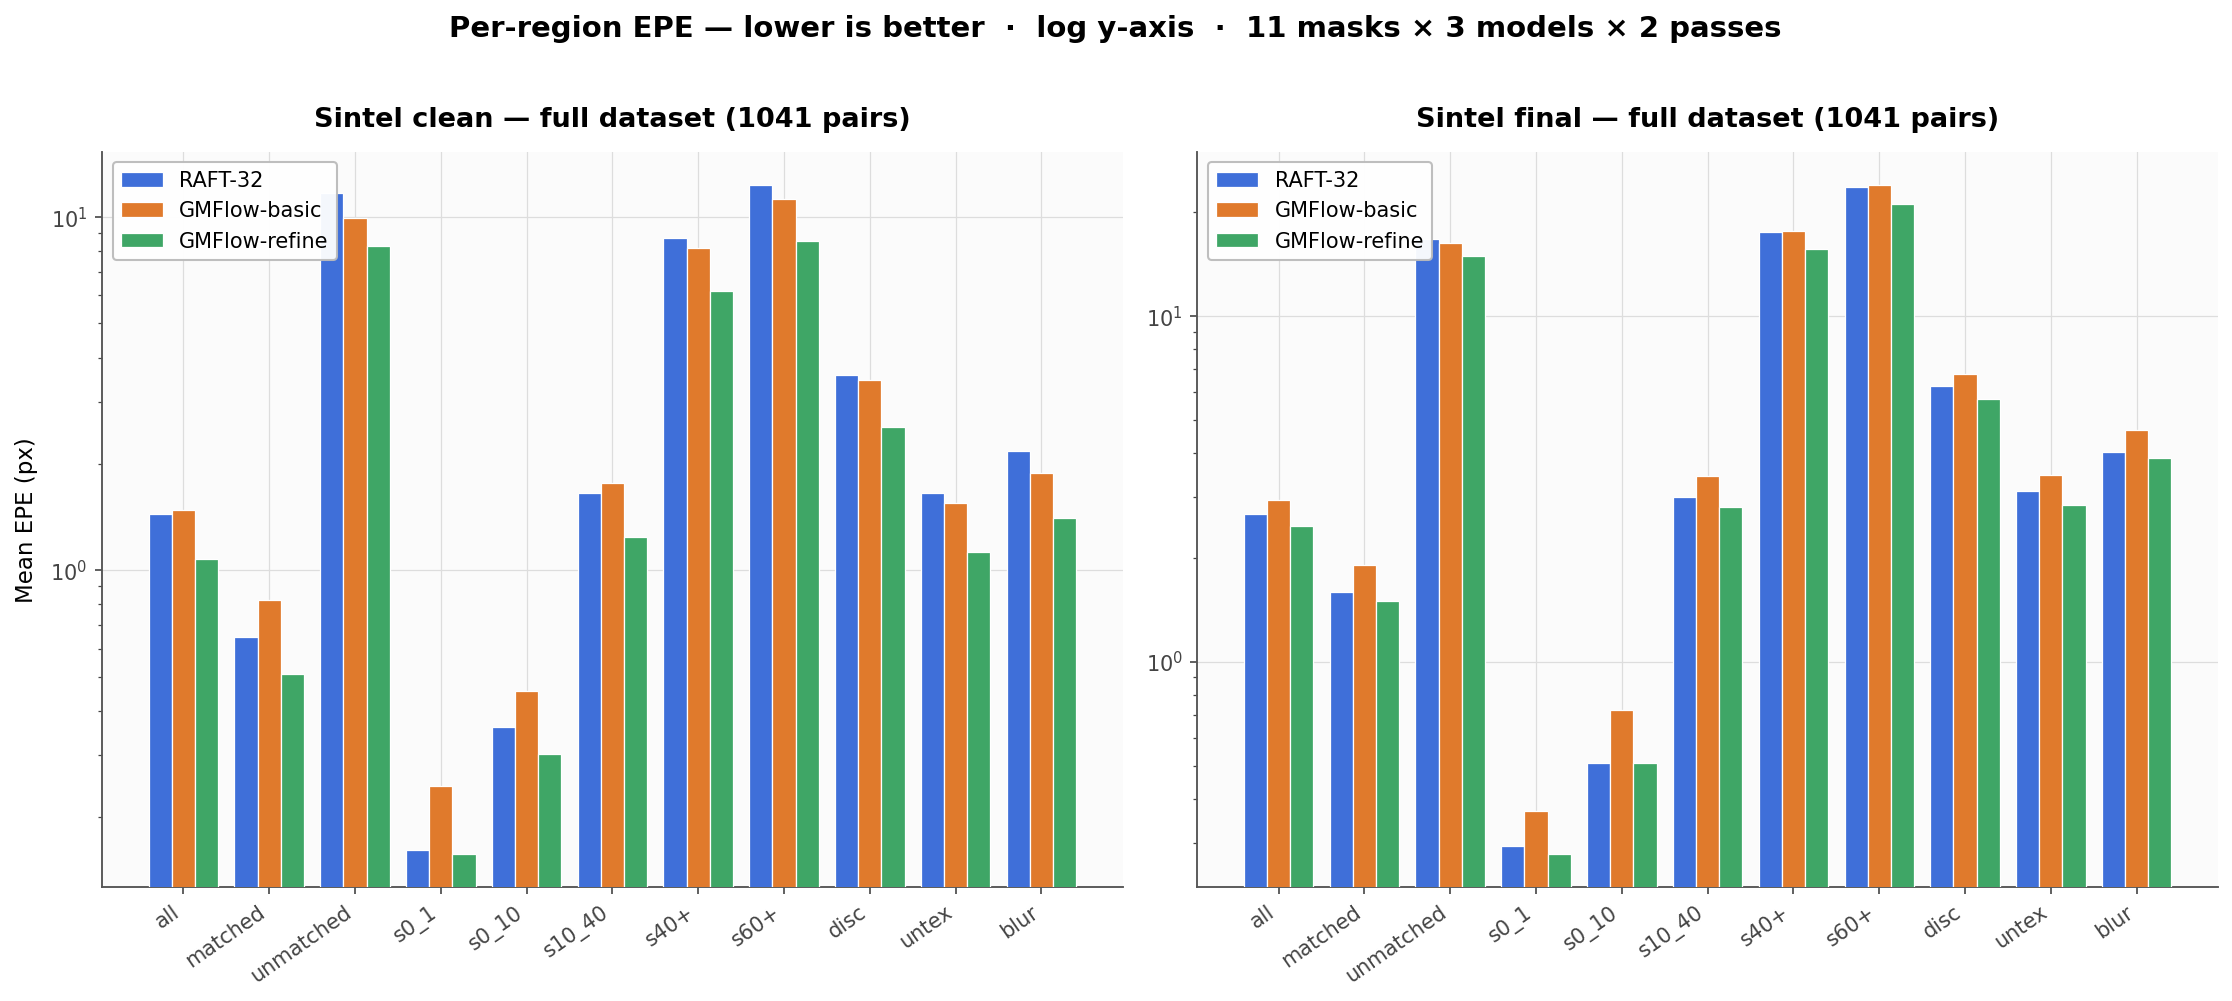
\includegraphics[width=0.96\linewidth]{figures/region_bars_full.png}
  \caption{Per-region EPE for all 11 masks, both passes (log y-axis).
    RAFT-32 (blue), GMFlow-basic (orange), GMFlow-refine (green).
    Refine is strongest overall, but several final-pass regions are
    statistically tied with RAFT.}
  \label{fig:region_bars}
\end{figure}

Figure~\ref{fig:region_bars} shows that errors are not uniform across
regions.  The s60+ bin (flow $>60$~px) carries the largest absolute
errors (RAFT 12.30~px clean), dwarfing the overall mean.  Disc-region
errors are roughly $2.5\times$ the global mean for all models, while
Untex errors are only marginally above global.  Blur pixels show a
surprising split: GMFlow-basic has \emph{lower} mean EPE on clean blur
pixels (1.88 vs.\ 2.18) but worse on every distributional metric
(Bad-1: 0.182 vs.\ 0.108; A95: 6.06 vs.\ 2.15 px).  On Final, where
the blurred-pixel fraction nearly triples (12.7\%~$\to$~34.6\%), RAFT
has the lower EPE point estimate (4.03 vs.\ 4.67), but the paired
sequence bootstrap marks this comparison NULL.  A moderate blur–motion
confound (Pearson~$= 0.644$) means the blur-mask signal partly reflects
fast-motion contamination rather than pure defocus.

\begin{figure}[!t]
  \centering
  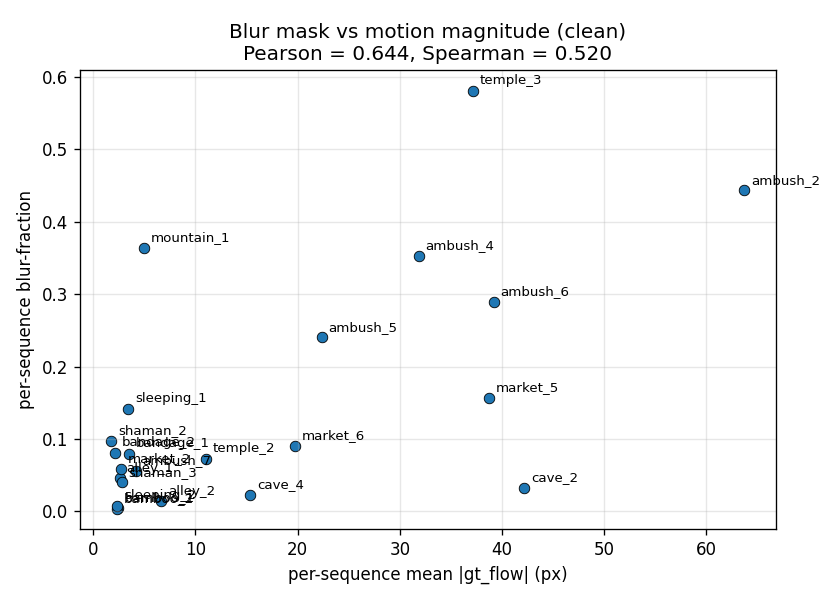
\includegraphics[width=0.76\linewidth]{figures/blur_motion_confound.png}
  \caption{Blur-mask fraction vs.\ mean GT-flow magnitude per Sintel-Clean
    sequence.  The positive correlation supports treating blur-region
    results as a mixed blur-plus-motion signal rather than a pure
    photometric-degradation measurement.}
  \label{fig:blur_confound}
\end{figure}

\begin{figure}[!t]
  \centering
  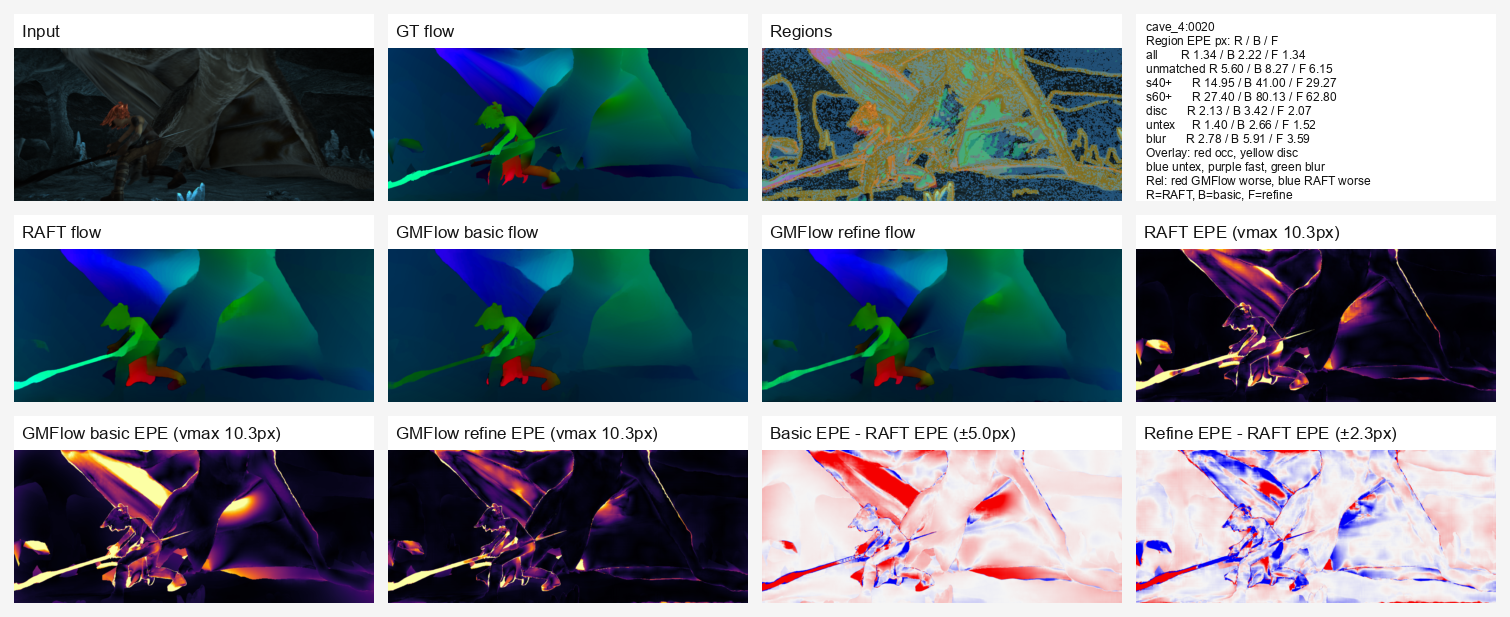
\includegraphics[width=0.98\linewidth]{figures/final_cave_4_panel.png}
  \caption{Qualitative failure panel on \texttt{final/cave\_4}.  The
    visualization compares input, GT flow, predicted flows, EPE maps, and
    residual differences, showing that aggregate EPE differences are
    concentrated around motion boundaries and difficult local structures.}
  \label{fig:qual_cave4}
\end{figure}

\subsection{Clean to Final degradation}

\begin{figure}[!t]
  \centering
  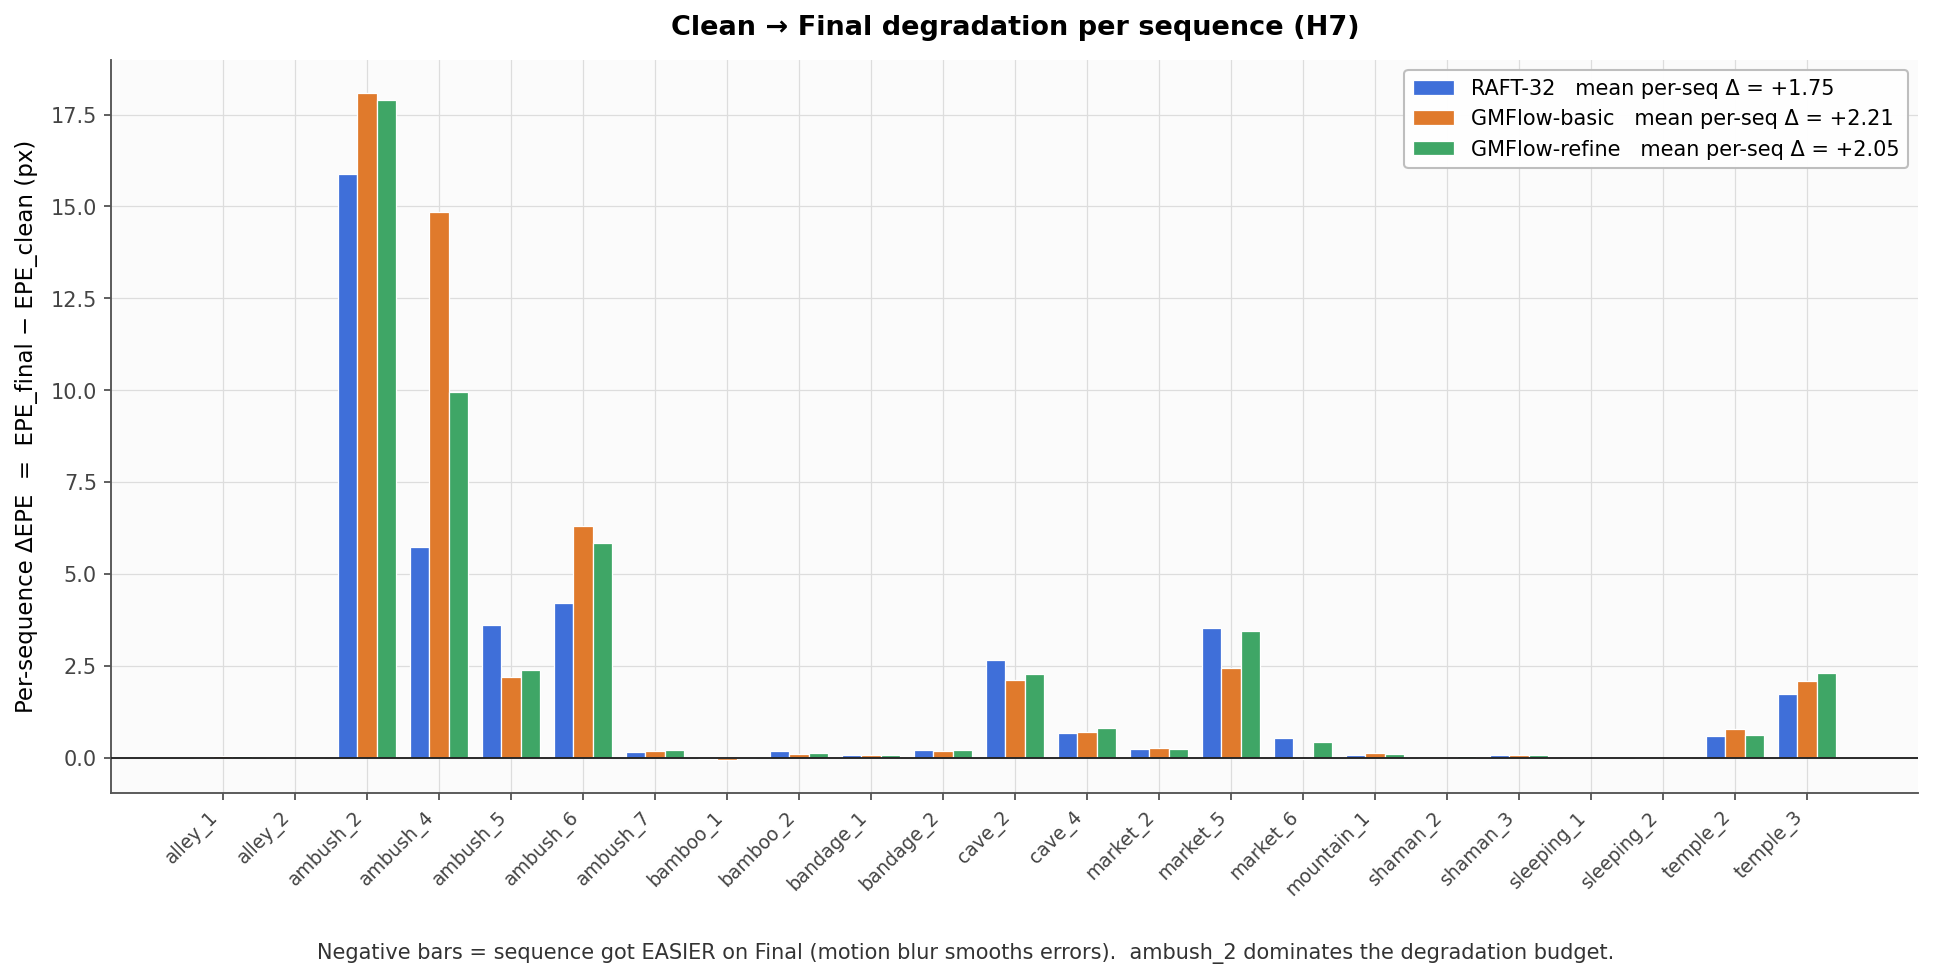
\includegraphics[width=0.96\linewidth]{figures/clean_to_final_delta.png}
  \caption{Per-sequence $\Delta$EPE (Final$-$Clean) for all 23 sequences
    and 3 models. \texttt{ambush\_2} dominates; a handful of slow
    sequences (bamboo, sleeping) show negative $\Delta$ (Final
    is \emph{easier} due to motion blur smoothing).}
  \label{fig:delta}
\end{figure}

RAFT degrades less overall: pixel-weighted $\Delta$EPE $= +1.23$ (RAFT)
vs.\ $+1.46$ (basic) vs.\ $+1.39$ (refine).  However this is
\emph{falsified} as a GMFlow advantage — the correct read is the
opposite: no GMFlow variant degrades less than RAFT.  An earlier
framing as a ``relative'' advantage was a denominator artifact
(GMFlow starts worse, so the same absolute $\Delta$ appears
proportionally smaller).

\texttt{ambush\_2} is the hardest sequence: median $\Delta$EPE of
$+16.88$~px (RAFT) and $+21.30$~px (GMFlow-basic).  \texttt{ambush\_4}
shows the largest inter-model gap: RAFT degrades $3\times$ less than
basic (median $\Delta$ 5.03 vs.\ 15.25~px) on this fast, high-blur
sequence.

\begin{figure}[!t]
  \centering
  \begin{subfigure}[t]{0.48\linewidth}
    \centering
    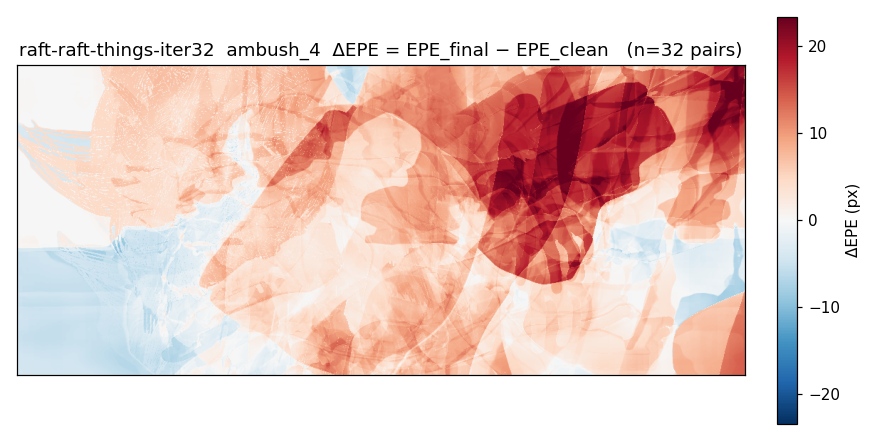
\includegraphics[width=\linewidth]{figures/delta_raft_ambush4.png}
    \caption{RAFT-32}
  \end{subfigure}
  \hfill
  \begin{subfigure}[t]{0.48\linewidth}
    \centering
    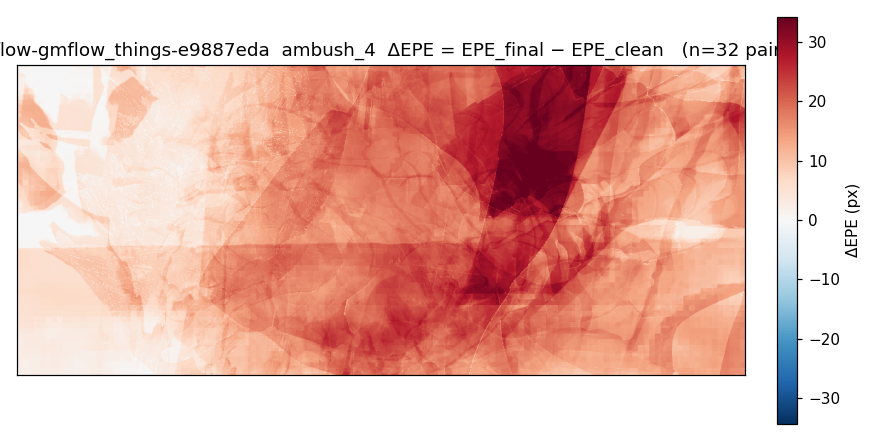
\includegraphics[width=\linewidth]{figures/delta_gmflow_basic_ambush4.png}
    \caption{GMFlow-basic}
  \end{subfigure}
  \caption{Spatial $\Delta$EPE maps on \texttt{ambush\_4}
    (Final$-$Clean).  GMFlow-basic shows a broader positive degradation
    field, matching the sequence-level gap in Figure~\ref{fig:delta}.}
  \label{fig:ambush4_delta_maps}
\end{figure}

\subsection{Boundary F1 sensitivity}

\begin{figure}[!t]
  \centering
  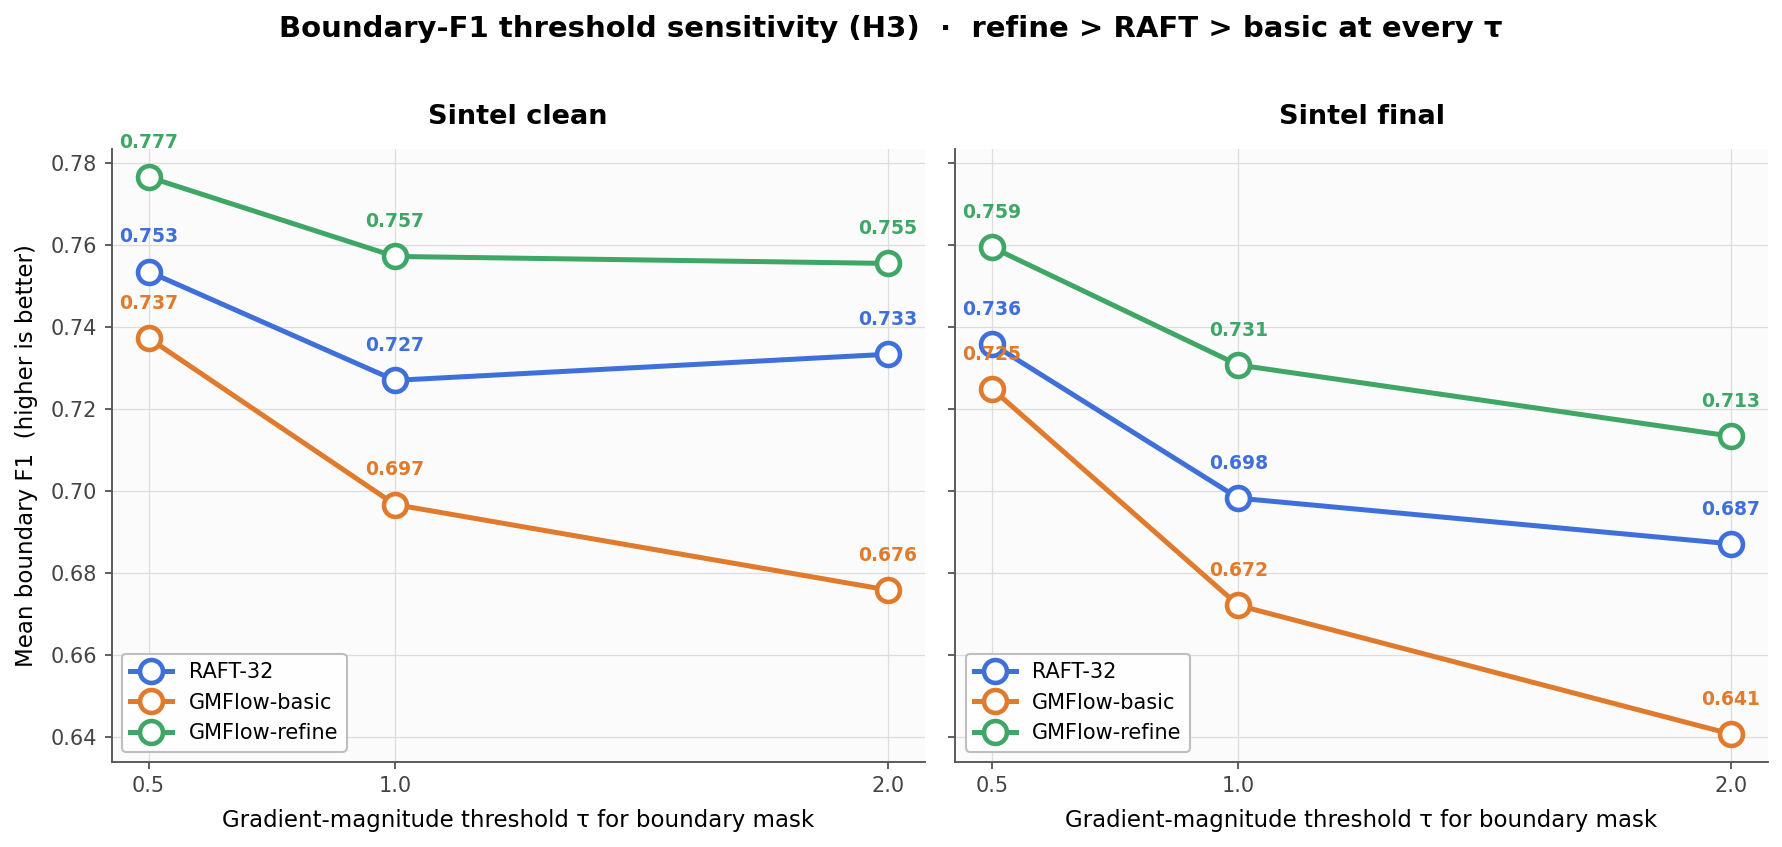
\includegraphics[width=0.82\linewidth]{figures/boundary_f1_sensitivity.png}
  \caption{Boundary F1 vs.\ disc-mask gradient threshold
    $\tau\in\{0.5,1.0,2.0\}$.  RAFT~$>$~basic at every $\tau$ and pass;
    refine~$>$~RAFT at every $\tau$ and pass.  No ranking flip.}
  \label{fig:f1}
\end{figure}

RAFT F1 = $0.727 / 0.698$ (clean/final) vs.\ basic $0.697 / 0.672$.
Refine wins at every threshold: $0.757 / 0.731$.  The ordering is
stable across $\tau\in\{0.5,1.0,2.0\}$ (absolute swing $\pm$3–4 pp),
confirming that RAFT's boundary advantage over \emph{basic} is robust
to the threshold choice — but that it is reversed by refine.

\subsection{Middlebury: cross-dataset generalization}

\begin{figure}[!t]
  \centering
  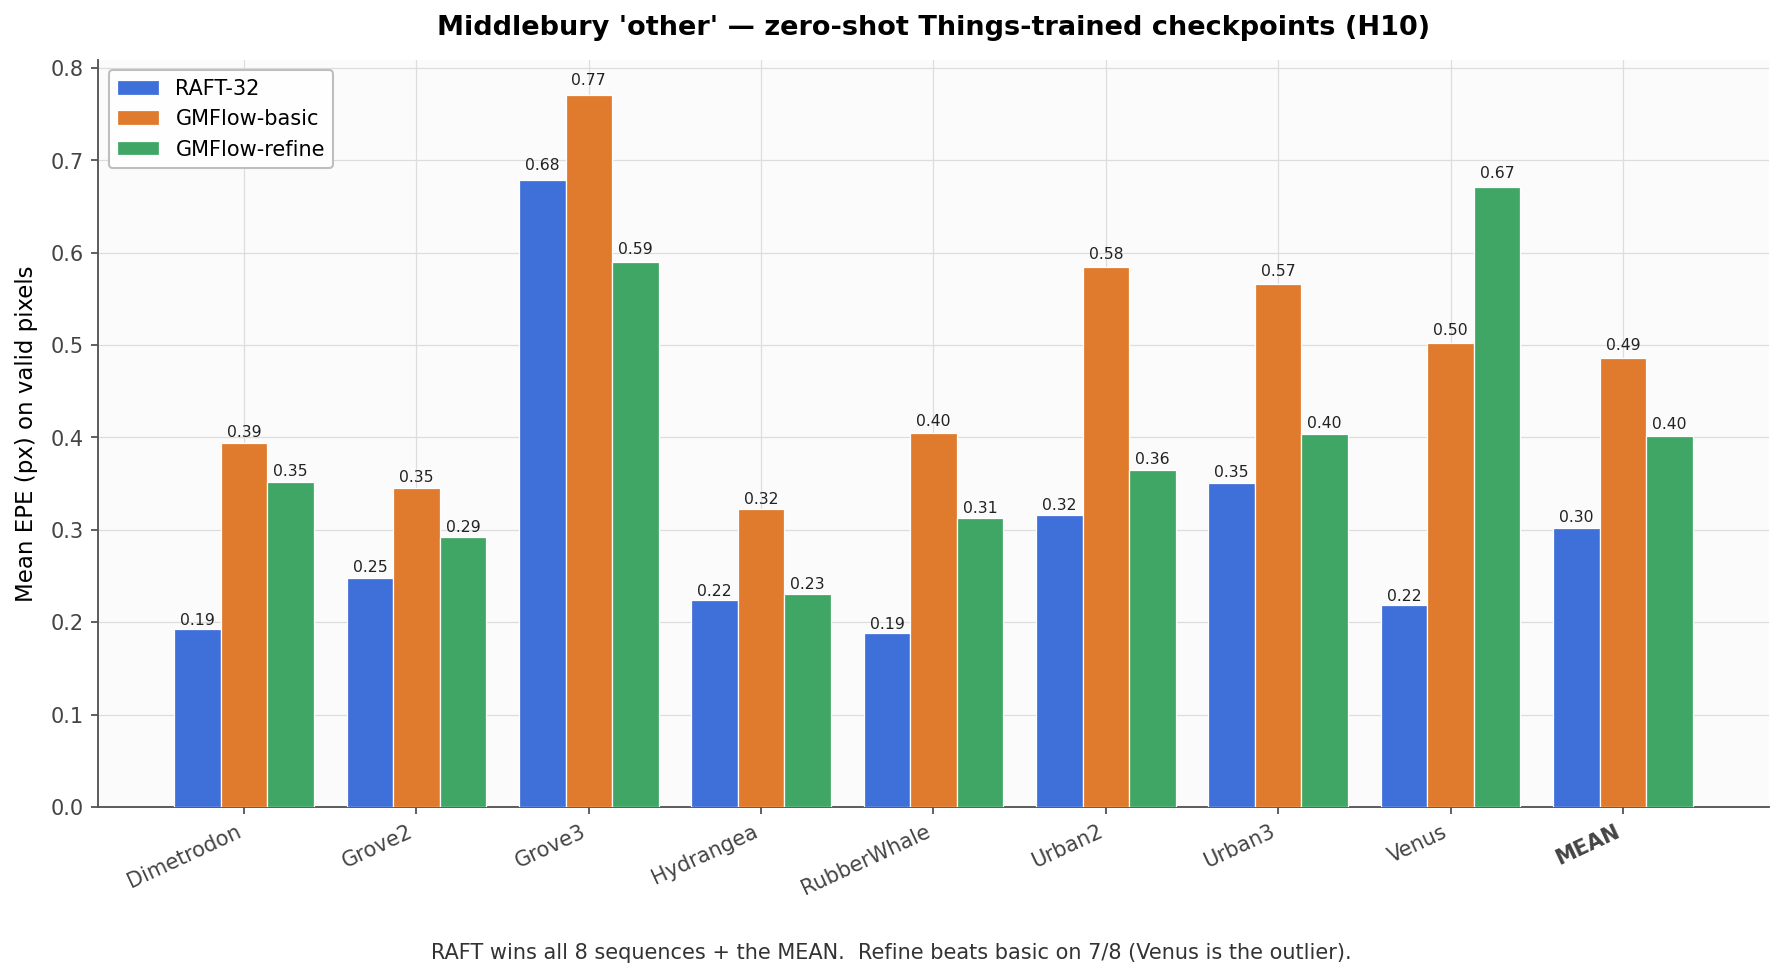
\includegraphics[width=0.96\linewidth]{figures/middlebury_per_seq.png}
  \caption{Middlebury per-sequence endpoint error (8 sequences + mean).
    RAFT wins all sequences; GMFlow-refine beats basic on 7/8.}
  \label{fig:middlebury}
\end{figure}

\begin{table}[htbp]
\centering
\caption{Middlebury mean EE and normalized cross-dataset scores.}
\label{tab:middlebury}
\small
\setlength{\tabcolsep}{5pt}
\begin{tabular}{lccc}
\toprule
Model & Mid.\ EE & Mid/Sintel-all & Mid/Sintel-$s_{0\text{-}10}$ \\
\midrule
RAFT-32      & \textbf{0.302} & \textbf{0.209} & \textbf{0.839} \\
GMFlow-basic & 0.486          & 0.328          & 1.066 \\
GMFlow-refine& 0.402          & 0.375          & 1.331 \\
\bottomrule
\end{tabular}
\end{table}

RAFT wins every Middlebury sequence.  R0.5 (fraction of pixels
missing the $0.5$~px target) averages $11.4\%$ for RAFT vs.\ $28.7\%$
for basic — over $2\times$ more pixels at sub-half-pixel accuracy.

Normalization matters for H10: using Mid/Sintel-all, GMFlow-basic's
normalized score is about 57\% higher than RAFT's; using the better
matched $s_{0\text{-}10}$ normalizer, it is about 27\% higher.
Middlebury motions are mostly $<10$~px, so the second normalizer is the
more comparable motion regime.
Refine's large normalized score (1.331) is \emph{not} Sintel
overfitting (both checkpoints are Things-trained); it reflects a
\textbf{motion-regime effect}: refine's extra capacity pays off on
Sintel's large-motion tail but buys little on Middlebury's all-small-motion
regime.

\subsection{Forward-backward derived occlusion}
Both models recover $\approx 0.60$ F1 / $0.43$ IoU of the GT Sintel
occlusion mask using forward-backward consistency
\cite{sundaram2010,meister2018}.  GMFlow is higher precision (0.752),
RAFT higher recall (0.564).  The quality of the
inferred occlusion mask and the EPE on occluded regions are
independent axes: similar F1 yet GMFlow has lower unmatched EPE
on clean, consistent with H4.

% ============================================================
\section{Hypothesis Verdicts}
% ============================================================

\begin{table}[htbp]
\centering
\caption{Summary of hypothesis verdicts. ``Basic'': vs.\ GMFlow-basic.
  ``Refine'': vs.\ GMFlow-refine.}
\label{tab:hypotheses}
\small
\setlength{\tabcolsep}{3pt}
\begin{tabular}{cllll}
\toprule
H & Claim & vs.\ Basic & vs.\ Refine & Verdict \\
\midrule
1 & GMFlow $>$ large displ. & NULL & \textbf{Supported} & Config/capacity effect \\
2 & RAFT $>$ sub-pixel & \textbf{Supported} & NULL & Config/capacity effect \\
3 & RAFT sharper boundaries & \textbf{Supported} & Falsified & Config/capacity effect \\
4 & GMFlow $>$ occlusions (clean) & \textbf{Supported} & \textbf{Supported} & Consistent \\
5 & Both adequate on untex & Supported & Supported & Confirmed \\
6 & RAFT iter trade-off & \multicolumn{2}{c}{\textbf{Supported}} & Monotone curve \\
7 & GMFlow $<$ Clean$\to$Final & \multicolumn{2}{c}{\textbf{Falsified}} & RAFT degrades less \\
8 & Weather vs.\ noise failure & \multicolumn{2}{c}{Not pursued} & Out of scope \\
9 & GMFlow VRAM blow-up & \multicolumn{2}{c}{Indicative only} & H/W contam. \\
10 & Unequal cross-dataset drop & \multicolumn{2}{c}{\textbf{Supported}} & RAFT generalizes better \\
\midrule
\end{tabular}
\end{table}

A recurring pattern in Table~\ref{tab:hypotheses}: several hypotheses
that held against GMFlow-basic are weakened or reversed against
GMFlow-refine.  H1, H2, and H3 are therefore best read as
\textbf{configuration/capacity-sensitive} rather than purely architectural:
the ``wins'' attributed to RAFT's iterative architecture do not all survive
when GMFlow is evaluated with its stronger refinement preset.  The more
stable findings are H4 (GMFlow handles occlusions better on clean, and
refine does so on both passes) and H10 (RAFT generalizes cross-dataset
better, attributable to the motion-regime effect rather than overfitting).

% ============================================================
\section{Discussion and Limitations}
% ============================================================

\textbf{What the models learned.}
RAFT's iterative ConvGRU is exceptionally sub-pixel precise — A50
$= 0.067$~px on clean, persistent even against refine.  This traces to
the correlation-volume lookup at $1/8$-pixel resolution combined with
many refinement steps.  GMFlow's convex upsampler leaves a soft
coarse-grid ($k/8$) concentration in the residual at small displacements,
explaining its $6\times$ larger A50.

\textbf{Architecture vs.\ capacity.}
The clearest takeaway from the three-way ablation is that many
``architectural'' conclusions from the RAFT-vs-basic comparison were
actually sensitive to configuration and capacity.  Refine, at 26\% better
EPE and only 10\% higher latency, is preferable when accuracy is prioritized,
while RAFT-32 remains slightly faster and more memory-efficient.  The
remaining architectural gap — RAFT's
sub-pixel precision and lower A50 — may disappear with a higher-capacity
GMFlow variant.

\textbf{Failure cases.}
\texttt{ambush\_2} and \texttt{ambush\_4} account for a disproportionate
share of both models' error budget: both sequences combine fast camera
motion with close-range foreground objects producing the largest optical
flow magnitudes in the dataset.  On these sequences GMFlow-basic
degrades $3\times$ more than RAFT on Final ($\Delta$EPE 21.30 vs.\ 16.88
for ambush\_2).

\textbf{Limitations.}
\begin{itemize}[leftmargin=1.4em,topsep=2pt,itemsep=1pt]
  \item \textbf{H9 not verified}: the resolution sweep at $\geq2\times$
    Sintel is contaminated by WSL2 unified-memory paging on the 4~GB
    GPU; allocated memory exceeds physical capacity, mixing O($N^2$)
    attention cost with PCIe transfer cost.  Re-run on a $\geq16$~GB
    physical-memory GPU is required.
  \item \textbf{RobustSpring out of scope}: H8 (weather vs.\ noise
    robustness, Oei et al.\ \cite{oei2026}) requires the RobustSpring
    corruption suite, which was descoped from this study.
  \item \textbf{Blur–motion confound}: the Laplacian-variance blur mask
    correlates with GT motion magnitude (Pearson $= 0.644$), so
    ``blur-region'' EPE differences partly reflect fast-motion
    contamination.
  \item \textbf{Derived motion-boundary mask}: Sintel's native
    \texttt{motion\_boundaries/} is not publicly distributed; we use a
    Sobel $+ 9{\times}9$ dilation approximation.  F1 is internally
    consistent but not directly comparable to papers using the native mask.
\end{itemize}

% ============================================================
\section{Conclusion}
% ============================================================

We evaluated RAFT and GMFlow in a zero-shot setting on MPI-Sintel and
Middlebury using 10 testable hypotheses, paired bootstrap CIs, and a
three-way ablation.  Key findings:

\begin{enumerate}[leftmargin=1.5em,topsep=2pt,itemsep=2pt]
  \item The headline ``RAFT wins on Sintel'' ($\Delta$EPE $= 0.038$) is
    \emph{statistically insignificant}.  RAFT's genuine wins are on
    matched pixels, sub-pixel accuracy (A50 $0.067$ vs.\ $0.411$~px),
    and cross-dataset generalization.
  \item GMFlow-refine outperforms RAFT-32 by 26\% EPE at 10\% higher
    latency ($652$ vs.\ $594$~ms), with significant clean-pass EPE wins
    on most masks and statistical ties in the two slowest speed buckets.
  \item RAFT degrades less Clean$\to$Final ($\Delta$EPE $+1.23$ vs.\
    $+1.46$~px); the hypothesis that GMFlow tolerates photometric
    degradations better is \textbf{falsified}.
  \item RAFT generalizes better to Middlebury (mean EE $0.302$ vs.\
    $0.486$; normalized $0.209$ vs.\ $0.328$) due to a motion-regime
    effect, not Sintel overfitting.
  \item Most H1/H2/H3 ``wins'' attributed to RAFT's architecture are
    configuration/capacity-sensitive and weaken against GMFlow-refine.
\end{enumerate}

Future directions: verify H9 on a $\geq16$~GB GPU, run the
RobustSpring corruption suite for H8, and test a higher-capacity
GMFlow-refine variant to determine whether the A50 gap persists.


\begingroup
\small
\begin{thebibliography}{9}

\bibitem{teed2020raft}
Z.~Teed and J.~Deng,
``RAFT: Recurrent All-Pairs Field Transforms for Optical Flow,''
\textit{European Conference on Computer Vision (ECCV)}, pp.~402--419, 2020.
\url{https://github.com/princeton-vl/RAFT}

\bibitem{xu2022gmflow}
H.~Xu, J.~Zhang, J.~Cai, H.~Rezatofighi, and D.~Tao,
``GMFlow: Learning Optical Flow via Global Matching,''
\textit{Proceedings of the IEEE/CVF Conference on Computer Vision and Pattern Recognition (CVPR)}, pp.~8121--8130, 2022.
\url{https://github.com/haofeixu/gmflow}

\bibitem{butler2012sintel}
D.~J.~Butler, J.~Wulff, G.~B.~Stanley, and M.~J.~Black,
``A Naturalistic Open Source Movie for Optical Flow Evaluation,''
\textit{European Conference on Computer Vision (ECCV)}, pp.~611--625, 2012.

\bibitem{baker2011}
S.~Baker, D.~Scharstein, J.~P.~Lewis, S.~Roth, M.~J.~Black, and R.~Szeliski,
``A Database and Evaluation Methodology for Optical Flow,''
\textit{International Journal of Computer Vision}, 92(1):1--31, 2011.
\url{https://doi.org/10.1007/s11263-010-0390-2}

\bibitem{oei2026}
V.~Oei, J.~Schmalfuss, L.~Mehl, M.~Bartsch, S.~Agnihotri,
M.~Keuper, A.~Bulling, and A.~Bruhn,
``RobustSpring: Benchmarking Robustness to Image Corruptions
for Optical Flow, Scene Flow and Stereo,''
\textit{International Conference on Learning Representations (ICLR)}, 2026.
\url{https://arxiv.org/abs/2505.09368}

\bibitem{horn1981}
B.~K.~P.~Horn and B.~G.~Schunck,
``Determining Optical Flow,''
\textit{Artificial Intelligence}, 17(1--3):185--203, 1981.
\url{https://doi.org/10.1016/0004-3702(81)90024-2}

\bibitem{sundaram2010}
N.~Sundaram, T.~Brox, and K.~Keutzer,
``Dense Point Trajectories by GPU-Accelerated Large Displacement Optical Flow,''
\textit{European Conference on Computer Vision (ECCV)}, pp.~438--451, 2010.
\url{https://lmb.informatik.uni-freiburg.de/Publications/2010/Bro10e/}

\bibitem{meister2018}
S.~Meister, J.~Hur, and S.~Roth,
``UnFlow: Unsupervised Learning of Optical Flow with a Bidirectional Census Loss,''
\textit{Proceedings of the AAAI Conference on Artificial Intelligence}, 32(1), 2018.
\url{https://doi.org/10.1609/aaai.v32i1.12276}

\end{thebibliography}
\endgroup

\end{document}
